\paragraph{Loss terms.} Table~\ref{tab:ablation} (upper block) varies the training objective on MNIST.
\begin{itemize}
\item \textbf{Percept-similarity term is essential.} Without it, training collapsed within the first 300 steps to currents below the rheobase, i.e.\ no phosphenes. The result is SSIM \AbNoPerSsim\ and accuracy \AbNoPerAcc, with a charge of essentially zero. With the decoder loss as the only objective, the gradient reaching a dark electrode passes through the sub-rheobase ReLU and the narrow threshold surrogate. Once most electrodes fall below threshold, that gradient vanishes.
\item \textbf{Decoder loss did not help at this scale.} Dropping it gave SSIM \AbNoRecSsim\ and accuracy \AbNoRecAcc, against \AbMainSsim\ and \AbMainAcc\ for the full objective.
\item \textbf{Charge cost is cheap.} Removing it raised summed charge from \AbMainCharge\ to \AbNoChgCharge\,\textmu C per phase without improving fidelity (SSIM \AbNoChgSsim).
\end{itemize}

\paragraph{Safety limits.} Removing the active-electrode cap and the charge cost, and raising the ceiling to 200\,\textmu A, gives better images: SSIM \AbUnconSsim\ against \AbMainSsim. The price is \AbUnconActive\ active electrodes instead of \AbMainActive\ and \AbUnconCharge\ against \AbMainCharge\,\textmu C of charge per phase, while recognition is unchanged (\AbUnconAcc\ against \AbMainAcc). For a device that must manage charge, heat and power, the constrained operating point is clearly preferable.

\paragraph{Electrode count and layout.} The lower block of Table~\ref{tab:ablation} and Fig.~\ref{fig:ablation} vary the implant.
\begin{itemize}
\item \textbf{Threads.} With 64 and 256 sites the learned encoder still beats intensity sampling on recognition: \AbThrAAcc\ against \AbThrAIntAcc, and \AbThrBAcc\ against \AbThrBIntAcc. Its relative advantage is largest when phosphenes are scarce.
\item \textbf{One Utah array (96 channels).} It covers only a $\sim$0.6$^\circ$ patch near $2^\circ$ eccentricity, so neither encoder can convey digits (accuracy \AbUtahAAcc\ learned, \AbUtahAIntAcc\ intensity). End-to-end training here also collapsed to no stimulation: the charge fell to essentially zero within 300 steps, the same dead-zone failure as above.
\item \textbf{Sixteen Utah arrays (1024 contacts).} They reach \AbUtahBAcc\ (learned) and \AbUtahBIntAcc\ (intensity); here intensity sampling is slightly better. Both are well below the same number of thread sites (\AbMainAcc), because the contacts cluster into 16 small patches of the visual field, where neighbouring phosphenes overlap.
\end{itemize}

\begin{figure}[t]
\centering
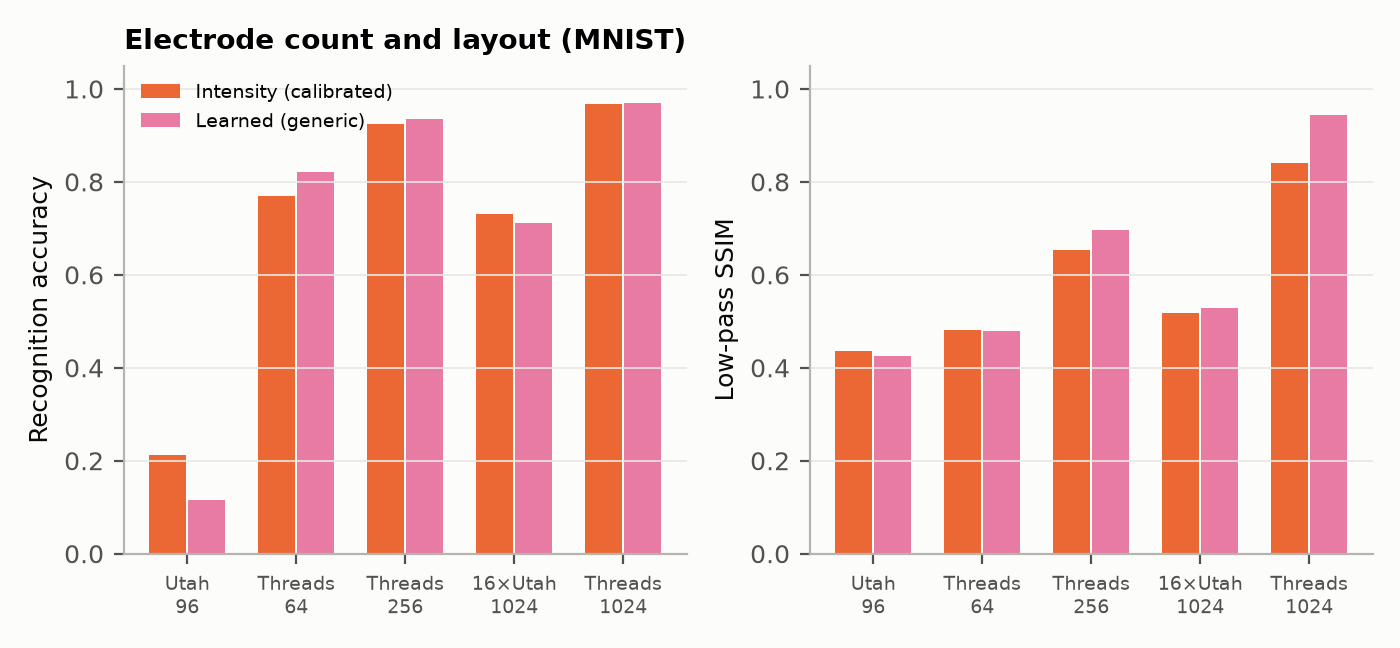
\includegraphics[width=\columnwidth]{fig_ablation_layouts.png}\\[2pt]
\IfFileExists{../results/figures/fig_adaptation_shots.png}{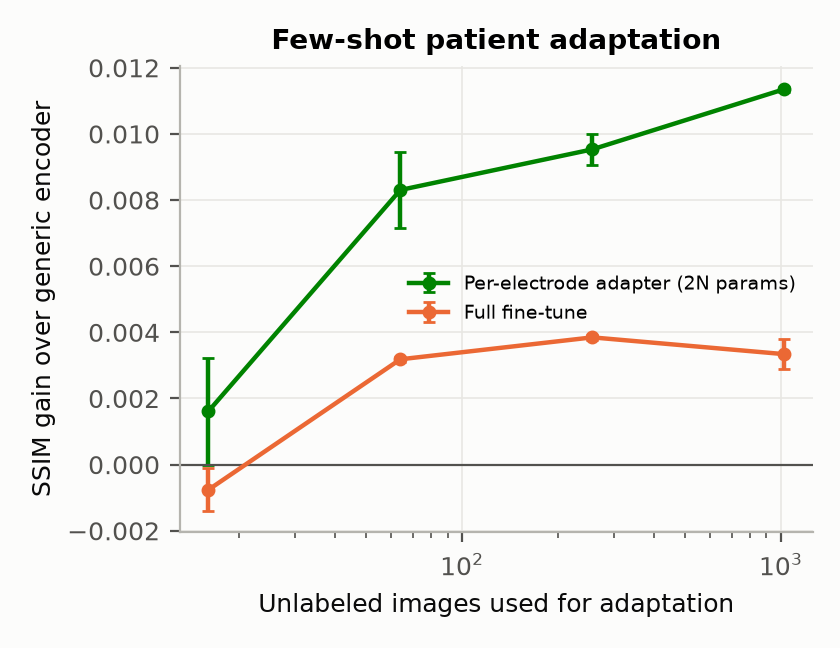
\includegraphics[width=0.75\columnwidth]{fig_adaptation_shots.png}}{}
\caption{\textbf{Top:} recognition and low-pass SSIM against electrode layout (MNIST, seed 0), learned encoder against intensity sampling. \textbf{Bottom:} SSIM gain from patient adaptation against the number of unlabeled images. MNIST, two held-out patients, 150 steps. With 64 or more images, adapter-only fine-tuning (2$N$ parameters) gains more than full fine-tuning.}
\label{fig:ablation}\label{fig:adapt}
\end{figure}
